\chapter{The fourth protocol - Removing The Overhead}
\label{chap:fourthProtocol}

% **************************** Define Graphics Path **************************
\ifpdf
    \graphicspath{{Chapter7/Figs/Raster/}{Chapter7/Figs/PDF/}{Chapter7/Figs/}}
\else
    \graphicspath{{Chapter7/Figs/Vector/}{Chapter7/Figs/}}
\fi

% ***** Main ****

\section{Introduction}
\label{sec:6intro}
In the last chapter, we developed a two-parties authentication protocol that
proves secure against a malicious client and does not leak any information to the
server (the main difference with the second protocol being that the server is not able to acquire the
value of the Hamming Distance between the registered and queried templates). This final variant aims to reduce both the communication
size and the computation time, while providing all the recommended security
features.
\begin{description}
\item[Reducing Communication Size] We observe that the main bottle neck of the
  communication is the size of the Stern-based ZKPs. We propose the
  following approach to replace old ZKPs:
  \begin{itemize}
  \item A Schnorr-based approach to replace the Stern-based one, to ensure that
    the noise in the ciphertext is small. This variant reduces the total
    communication rounds from \(log_{3/2}(FAR)^{-1}\) to just 1. Given a typical
    value of $FAR = 10^{-4}$, such improvement reduces the total number of
    communication rounds from $\approx 22$ to $1$.
  \item A challenge-response protocol to prove the binary format of the
    plaintext.
    % The protocol can be summarized as follows:
    % \begin{enumerate}
    % \item The server samples \(r_{1}, r_{2} \randomsample R_{q}\) and computes
    %   \(ch = enc(r_{1}*Q*(1-Q) + r_{2}) + enc(0,r)\) and sends \(ch\) to the
    %   client.
    % \item The client decrypts the result and sends back \(rsp\).
    % \item The server accepts the response if and only if \(rsp = r_{2} \)
    % \end{enumerate}
    % We remark that the first operation needs to be computed bit-wise, that means
    % we need to change the ciphertext packing method (the CRT-packing
    % \cite{smart2014fully} can support this requirement).
  \end{itemize}
\item[Reducing Computation Time.] By applying a new ciphertext packing
  method, we can effectively change the way of computing the Hamming Distance by
  summing up the bits of the XOR result of 2 bitstrings instead of computing their
  inner product. Therefore, enforcing this approach, we lower the computation time by performing
  additions only (without any homomorphic multiplication). The cost of this change
  is a set of switching keys for homomorphic rotation operations, which are
  generated during the enrollment process. Additionally, we introduce the
  application of state-of-the-art \textit{Secure-Multiparty-Protocol}
  techniques, such as \textit{Garbled Circuit} and \textit{Oblivious Transfer} into
  the lattice-based context, to further improve both the computation time and
  the communication size overhead implied by previous ZKP protocols.
\end{description}
This approach is practical because it moves a major part of the overhead to the
one-time set up phase of the protocol (the enrollment stage). Our results show
that the protocol can work efficiently during authentication stage. The
technique maybe generalized to similar multi-stage protocols.

\section{Reducing the communication overhead}
\label{sec:6challenge}

\subsection{The Schnorr-based ZKP}
\label{sec:zkpschnorr}
In the previous variants of the protocol, the critical module required to
provide active security against a malicious client is the binary message format
prover. Specifically, Alice sends a ciphertext \(C\) of a bitstring to Bob. Bob
is supposed to use a homomorphic encryption technique to process \(C\). Before
doing so, Bob might want to make sure that \(C\) is an encryption of a bitstring
(and not something else). In the last chapter, we used the Stern-based Zero Knowledge
Proof technique for this step, and it was shown that the communication size for
this is large due to the soundness error $2/3$ for each round of the ZKP (the
repetition of many proof-rounds being required to obtain a specific security
level). This chapter investigates another alternative to ZKP, exhibiting a better
soundness error of $1/n$ within one round of proof only, where $n$ is typically
the required parameter: the Schnorr-based ZKP technique. We first recall some
notation and concepts to be used in the chapter.

We denote a language $\mathcal{L} \subseteq \left\{ 0,1 \right\}^* $ having a
witness relationship
$R \subseteq \left\{ 0,1 \right\}^* \times \left\{ 0,1 \right\}^*$ if
$x \in \mathcal{L} \iff \exists (x,w) \in R$, where $w$ is a witness for
$x \in \mathcal{L}$.We discuss a definition of the sigma protocol from
\cite{benhamouda2014better}, which can be adapted to suit the techniques we use
in our project.

\begin{definition}
  \label{def:zkp-sum-protocol}
  Let (P,V) be a two-party protocol, where $V$ is PPT, and let
  $\mathcal{L},\mathcal{L'} \subseteq \left\{ 0,1 \right\}^*$ be languages with
  witness relations $\mathcal{R},\mathcal{R'}$ such that $\mathcal{R}
  \subseteq \mathcal{R'}$. $(P,V)$ is called a $\sum'-$protocol for
  $\mathcal{L}, \mathcal{L'}$ with completeness error $\alpha$, challenge set
  $\mathcal{C}$, public input $x$ and private input $w$, if and only if it
  satisfies the following conditions:
  \begin{itemize}
  \item Three-move form: The protocol is of the following form: The
    prover $P$, on input $(x,w)$, computes a commitment $t$ and sends it
    to $V$. The verifier $V$, on input $x$, then draws a challenge
    $c \randomsample \mathcal{C}$ and sends it to P. The prover sends a
    response $s$ to the verifier. Depending on the protocol transcript
    $(t,c,s)$, $V$ accepts or rejects the proof.
  \item Completeness: Whenever $(x,w) \in \mathcal{R}$, the verifier
    $V$ accepts with probability at least $1 - \alpha$.
  \item Special Soundness: There exists a PPT algorithm E, also known as
    the knowledge extractor, that takes two accepted transcript
    $(t,c',s')$,$(t,c'',s'')$ satisfying $c' \neq c''$ as inputs and
    output $w'$ such that $(x,w') \in \mathcal{R'}$.
  \item Special honest-verifier zero-knowledge (HVZK): There exists a
    simulator $S$, which is a PPT
    algorithm taking $x\in \mathcal{L}$ and $c \in \mathcal{C}$ as
    inputs and outputs $(t,s)$ so that the triple $(t,c,s)$ is
    indistinguishable from a valid protocol transcript.
  \end{itemize}
\end{definition}

This definition is different from the original sigma protocol in 2 ways.
First, it allows a completeness error $\alpha$ instead of perfect completeness
($\alpha=0$ in the original protocol).
Second, a second language $\mathcal{L}$ is introduced, with witness relation
$\mathcal{R} \subseteq \mathcal{R'}$: A prover knows a witness in $\mathcal{R}$
is guaranteed privacy, but the verifier is only ensured that the $P$ only knows
a witness for $\mathcal{R'}$. We refer to this as \emph{soundness gap}, if the
gap is small enough, it implies security guarantee for higher level applications
($\mathcal{R} = \mathcal{R'}$ in the original protocol).

The original Schnorr ZKP protocol \cite{schnorr1989efficient} can be used to prove
knowledge of a discrete logarithm (DL). It is described informally as in
Figure \ref{fig:schnorrProtocol}

\begin{figure}[htbp!] 
\centering \procedure{Schnorr Protocol for DL}{
  \textbf{Prover} \> \> \textbf{Verifier}\\
  (x = \log_g h) \> \> \\
  u \randomsample \mathbb{Z}_n \> \> \\
  t \gets g^u \> \sendmessageright*{t} \> \\
  \> \sendmessageleft*{c} \> c \randomsample \mathbb{Z}_n \\
  s \gets u + cx \> \sendmessageright*{s} \> \\
  \> \> g^s \stackrel{?}{=} ah^c
}
\caption{Schnorr Protocol}
\label{fig:schnorrProtocol}
\end{figure}

The soundness property of Schnorr's protocol can be argued by assuming that if a prover
is able to answer correctly at least two challenges $c$ and $c'$ (with
$c \neq c'$) after committing to an announcement $t$, then he would be able to infer
a solution for the hard problem of discrete log $x = \log_{g}h$. Hence,
intuitively, if the prover can answer at most one challenge correctly, the
probability of success is bounded by $1/n$, which can be negligibly small. The
Zero Knowledge property (against a semi-honest Verifier) was proved by showing
that the real conversation
$\{(t,c,s): u,c \randomsample \mathbb{Z}_{n}; t \gets g^{u}; s \gets u + cx\}$
and the simulated conversation
$\{(t,c,s): c, s \randomsample \mathbb{Z}_{n}; t \gets g^{s}h^{-c}\}$ are
identical (each valid conversation $(t;c;s)$ occurs with probability $1/n^{2}$
in both distributions).

In the work of \cite{benhamouda2014better}, the authors proposed a variant of
such technique to prove knowledge of small RLWE secret \textbf{s} and noise
\textbf{e} (in short, we mean that
$\norm{\mathbf{s}}, \norm{\mathbf{e}} \leq \bigO{n \alpha}$ for noise parameter
$\alpha$), where $(\mathbf{a}, \mathbf{y} = \mathbf{as} + \mathbf{e})$ is the
verifier's input and $(\mathbf{s,e})$ is the prover's witness input (see Figure
\ref{fig:benhamoudaProtocol})
% In the work of \cite{benhamouda2014better}, the authors proposed a variant
% of such technique to prove LWE-secrets (Figure \ref{fig:benhamoudaProtocol} )
\begin{figure}[htbp!] 
\centering \procedure{Benhamouda Protocol for RLWE}{
  \textbf{Prover} \> \> \textbf{Verifier}\\
  \mathbf{r}_s, \mathbf{r}_e \randomsample D_{\bigO{\sqrt{n}\alpha}} \> \> \\
  t = a \mathbf{r}_s + \mathbf{r}_e \> \> \\
  (c_{aux}, d_{aux}) = aCommit(t) \> \sendmessageright*{c_{aux}} \> \\
  \> \sendmessageleft*{c} \> c \randomsample \{0, \dots, 2n -1\}\\
  \mathbf{s}_s = \mathbf{r}_s + X^c s \> \> \\
  \mathbf{s}_e = \mathbf{r}_e + X^c e \> \> \\
  \> \sendmessageright*{t, d_{aux}, (\mathbf{s}_s, \mathbf{s}_e)} \> X^cy + t \stackrel{?}{=} a \mathbf{s}_s + \mathbf{s}_e \\
  \> \> aCOpen(t, c_{aux}, d_{aux}) \stackrel{?}{=} \text{accept}\\
  \> \> \norm{\mathbf{s}_s}, \norm{\mathbf{s}_e} \leq \bigO{n\alpha}
}
\caption{Proof of knowledge of RLWE secrets}
\label{fig:benhamoudaProtocol}
\end{figure}

Where $y = as + e$, and $s, e \randomsample D_{\alpha}$. In the protocol, the
prover is able to convince a verifier that it knows short secrets for twice the
public input (in short, we mean that $\norm{s},\norm{e} \leq \bigO{n\alpha}$).
We present an adaption of this ZKP protocol to prove the plaintext knowledge of
BV cryptosystems. Recall that given $\mathbf{(sk,pk) = (s,(p_0,p_1))}$ where
$\mathbf{s} \in \chi_{\beta_0}^n$, $\mathbf{p_0,p_1} \in R_q$ , a message
$\mathbf{m} \in R_t$ is encrypted by
$\enc{\mathbf{m}} := \mathbf{(c_0, c_1)} = (\mathbf{p_0u} + t\mathbf{f + m,
  p_1u} + t\mathbf{g)}$. The protocol (Figure \ref{fig:belhamoudaProtocol}) is
an AND composition of 2 ZKPs that prove 2 relations: the secret key $\mathbf{s}$
corresponds to the public key $\mathbf{(p_0,p_1)}$, i.e.,
$\mathbf{p_0 = -p_1s} - t\mathbf{e_0}$, and the ciphertext $\mathbf{(c_0,c_1)}$
is well-formed and encrypts the message $\mathbf{m}$, that is,
$\mathbf{c_0 + c_1s} = \mathbf{m} + t\mathbf{e}$, with
$\norminf{\mathbf{e}} \leq \beta$. Note that the protocol guarantees by $V$
that $P$ knows the plaintext encrypted in $2\mathbf{c_0}$

\begin{figure}[htbp!] 
  \centering \procedure{Schnorr-based ZKP for BV}{
    \textbf{Prover} \> \> \textbf{Verifier}\\
    \mathbf{r_s,r_{e_0}} \randomsample D_{\beta_0} \> \> \\
    \mathbf{r_e} \randomsample D_{\beta} \> \> \\
    \mathbf{r_m} \randomsample D_{t} \> \> \\
    \mathbf{t_c} = \mathbf{-c_1r_s} + t\mathbf{r_e + r_m} \> \> \\
    \mathbf{t_k} = \mathbf{-p_1r_s} - t\mathbf{r_{e_0}} \> \> \\
    (c_{aux}, d_{aux}) = aCommit(\mathbf{t_c,t_k}) \>
    \sendmessageright*{c_{aux}} \> \\
    \> \> c \randomsample \mathcal{C} = \left\{ 0,\dots, 2n -1  \right\}\\
    \>  \sendmessageleft*{c} \> \\
    \mathbf{s_s = r_s + x^cs} \> \> \\
    \mathbf{s_e = r_e + x^ce} \> \> \\
    \mathbf{s_m = r_m + x^cm} \> \> \\
    \mathbf{s_{e_0} = r_{e_0} + x^ce_0} \> \> \\
    \> \sendmessageright*{d_{aux}, \mathbf{t_c, t_k, s_s, s_e, s_m,
        s_{e_0}}} \> \\
    \> \> \mathbf{x^cc_0} + \mathbf{t_c} \stackrel{?}{=} -\mathbf{c_1s_s}
    +t\mathbf{s_e} + \mathbf{s_m}\\
    \> \> \mathbf{x^cp_0} + \mathbf{t_k} \stackrel{?}{=} -\mathbf{p_1s_s}
    -t\mathbf{s_{e_0}}\\
    \> \> aCOpen(\mathbf{t_c, t_k}, c_{aux}, d_{aux}) \stackrel{?}{=} accept
    \\
    \> \> \norm{s_s}, \norm{s_{e_0}} \leq 2\beta_0 \\
    \> \> \norm{s_e} \leq 2\beta \\
    \> \> \norm{s_m} \leq 2t
  }
  \caption{ZKP for BV cryptosystem relation}
  \label{fig:belhamoudaProtocol}
\end{figure}


\begin{theorem}
  Figure (\ref{fig:belhamoudaProtocol}) is a $\sum'$-Protocol for the following
  relations:
  \begin{equation}
    \label{equ:zkp_relation1}
    \begin{multlined}
      \mathcal{R} = \{ \left( \mathbf{c_0,c_1,p_0,p1},t \right), (\mathbf{m,
        s, e, e_0}): \mathbf{c_0 = -c_1s} + t\mathbf{e} +
      \mathbf{m}
      \wedge \mathbf{p_0 = -p_1s} - t\mathbf{e_{0}} \\
      \wedge \norminf{\mathbf{m}} \leq t
      \wedge \norm{\mathbf{e}} \leq \beta \wedge
      \norm{\mathbf{s}},\norm{\mathbf{e_0}} \leq \beta_0 \}
    \end{multlined}
  \end{equation}

  \begin{equation}
    \label{eq:zkp_relation2}
    \begin{multlined}
      \mathcal{R'} = \{ \left( \mathbf{c_0,c_1,p_0,p1},t \right), (\mathbf{m,
        s, e, e_0}): \mathbf{2c_0 = -2c_1s} + 2t\mathbf{e} + 2\mathbf{m} \wedge
      \mathbf{2p_0 = -2p_1s} - 2t\mathbf{e_{0}} \\
      \wedge
      \norminf{\mathbf{2m}} \leq 2t
      \wedge \norm{\mathbf{2e}} \leq 2\beta \wedge
      \norm{\mathbf{2s}},\norm{\mathbf{2e_0}} \leq 2\beta_0 \}
    \end{multlined}
  \end{equation}


  The protocol has a knowledge error of $\frac{1}{2n}$ and a completeness
  error of $1 - \frac{1}{M}$.

  \label{theo:BVZKPBenhamouda}
\end{theorem}

\begin{proof}
  We prove the properties specified in Definition \ref{def:zkp-sum-protocol} following the proof from \cite{benhamouda2014better}.
  \begin{description}
  \item[Completeness.] If the Prover $P$ sends a response, the following becomes the case:
    \begin{align*}
      -\mathbf{c_1s_s} + t\mathbf{s_e} + \mathbf{s_m} &= -\mathbf{c_1(r_s +
                                                        x^cs)} + t(\mathbf{r_e + x^ce}) + \mathbf{r_m + x^cm} \\
                                                      &= \mathbf{x^c}(-\mathbf{c_1s} +t\mathbf{e} + \mathbf{m})
                                                        -\mathbf{c_1r_s} + t\mathbf{r_e} + \mathbf{r_m}\\
                                                      &=\mathbf{x^cc_0} + \mathbf{t_c}
    \end{align*}
    Similarly
    \begin{align*}
      -\mathbf{p_1s_s} -t\mathbf{s_{e_0}} &= -\mathbf{p_1(r_s +
                                            x^cs) - t(\mathbf{r_{e_0} + x^ce_0})}\\
                                          &= \mathbf{x^c}(\mathbf{-p_1s} - t\mathbf{e_0}) -\mathbf{p_1r_s}
                                            -t\mathbf{r_{e_0}} \\
                                          &= \mathbf{x^cp_0 + t_k}
    \end{align*}
    Regarding norms, we have $\norm{\mathbf{s_s}} = \norm{\mathbf{r_s +
        x^cs}} \leq
    \norm{\mathbf{r_s}} + \norm{\mathbf{s}} \leq 2\beta_0$, and
    the same for $\mathbf{\norm{s_e}, \norm{s_m}, \norm{s_{e_0}}}$.
  \item [Special Soundness.] Before proving this property, we describe the
    following technical lemma 
    \begin{lemma}
      Let n be a power of 2 and let $0 <i,j< 2n-1$. Then, $2(x^i -
      x^j)^{-1} \mod (x^n +1)$ only has coefficients in $\left\{ -1,
        0, 1
      \right\}$.
      \label{lem:speicalBinomial}
    \end{lemma}
    Assume that a dishonest prover does not know 'small'
    $2\mathbf{s}, 2\mathbf{e}, 2\mathbf{m}$ and $2\mathbf{e_0}$ and can
    output different accepted transcripts of a same commitment: $(c_{aux}, c',
    (d'_{aux},\mathbf{t'_c, t'_k, s'_s, s'_e, s'_m, s'_{e_0}}))$ and
    $(c_{aux}, c'', (d''_{aux}, \mathbf{t''_c, t''_k, s''_s, s''_e,
      s''_m, s''_{e_0}}))$. From the binding property of the auxiliary
    commitment scheme \cite{pedersen1991non}, we have $\mathbf{t'_c = t''_c := t_c}$
    and $\mathbf{t'_k = t''_k := t_k}$. As the transcripts pass the
    checks by the verifier, it appears that:
    \begin{align*}
      &\begin{cases}
        \mathbf{x^{c'}c_0 + t_c} = -\mathbf{c_1s'_{s}} +
        t\mathbf{s'_{e}+ s'_{m}}
        \\
        \mathbf{x^{c'}p_0} + \mathbf{t_k} = -\mathbf{p_1s'_s}
        -t\mathbf{s'_{e_0}}
      \end{cases} \&
      &\begin{cases}
        \mathbf{x^{c''}c_0 + t_c} = -\mathbf{c_1s''_{s}} +
        t\mathbf{s''_{e}+ s''_{m}}
        \\
        \mathbf{x^{c''}p_0} + \mathbf{t_k} = -\mathbf{p_1s''_s}
        -t\mathbf{s''_{e_0}}
      \end{cases}
    \end{align*}
    By subtracting the equations we get:
    \begin{align*}
      \begin{cases}
        \mathbf{c_0(x^{c'} - x^{c''})} = -\mathbf{c_1}(\mathbf{s'_s
          - s''_s}) + t\mathbf{(s'_e - s''_e)} +(\mathbf{s'_m -
          s''_m})\\
        \mathbf{p_0(x^{c'} - x^{c''})} = -\mathbf{p_1(s'_s - s''s)}
        - t\mathbf{(s'_{e_0} - s''_{e_0})}
      \end{cases}
    \end{align*}
    Multiplying by $2(\mathbf{x^{c'} - x^{c''}})^{-1}$:
    \begin{align*}
      \begin{cases}
        \mathbf{2c_0} = -\mathbf{c_1}2(\mathbf{s'_s
          - s''_s})(\mathbf{x^{c'} - x^{c''}})^{-1} + t2\mathbf{(s'_e -
          s''_e)}(\mathbf{x^{c'} - x^{c''}})^{-1} +2(\mathbf{s'_m -
          s''_m})(\mathbf{x^{c'} - x^{c''}})^{-1}\\
        \mathbf{p_0} = -\mathbf{p_12(s'_s - s''_s)}(\mathbf{x^{c'} - x^{c''}})^{-1}
        - t2\mathbf{(s'_{e_0} - s''_{e_0})}(\mathbf{x^{c'} - x^{c''}})^{-1}
      \end{cases}
    \end{align*}
    Let $2\hat{\mathbf{s}} = 2(\mathbf{s'_s -
      s''_s})(\mathbf{x^{c'}-x^{c''}})^{-1} $, $2\hat{\mathbf{e}} =
    2\mathbf{(s'_e - s''_e)(x^{c'} - x^{c''})^{-1}}$,
    $2\hat{\mathbf{e_0}} = 2\mathbf{(s'_{e_0}-s''_{e_0})(x^{c'} -
      x^{c''})^-1}$ and $2\hat{\mathbf{m}}=2\mathbf{(s'_m -
      s''_m)(x^{c'} - x^{c''})^{-1}}$. Applying the result from Lemma
    \ref{lem:speicalBinomial}, we see that $P$ knows the 'small' secrets
    $\norm{\hat{\mathbf{2s}}} < 2\beta_0$, $\norm{\hat{\mathbf{2e}}} <
    2\beta_0$, $\norm{\hat{\mathbf{2e_0}}} < 2\beta$ and
    $\norm{\hat{\mathbf{2m}}} < 2t$ that can pass the verifier's checks.
    This contradicts our assumption. In other words, the prover has to
    know the secret to pass the proof with probability
    $\frac{1}{2n}$.
  \item [Honest Verifier Zero-Knowledge.] The verifier can use a
    simulator $S$ to reproduce the
    protocol transcript as follows:
    \begin{itemize}
    \item $V$ samples $c \randomsample \mathcal{C}$
    \item With probability 1/M, $S$ chooses $\mathbf{s_s, s_{e_0}}
      \randomsample D_{\beta_0}$, $\mathbf{s_e} \randomsample
      D_{\beta}$ and $\mathbf{s_m} \randomsample D_t$.
    \item $S$
      computes $\mathbf{t_c} = \mathbf{-c_1s_s} + t\mathbf{s_e} +
      \mathbf{s_m} - \mathbf{x^cc_0}$ and $\mathbf{t_k} =
      -\mathbf{p_1s_s} -t\mathbf{s_{e_0}} - \mathbf{x^cp_0}$ and
      $(c_{aux}, d_{aux}) \leftarrow aCommit(\mathbf{t_c,t_k})$.
    \item $S$ outputs $(c_{aux}, c, (\mathbf{(t_c,t_k)},
      d_{aux},(\mathbf{s_s,s_{e_0},s_e,s_m})))$
    \end{itemize}
    The distribution of $\mathbf{(s_s, s_{e_0}, s_e, s_m)}$ does not depend on
    real secrets. Hence, the simulated transcript becomes insdistinguishable
    from the real one.
  \end{description}
\end{proof}

\subsection{The challenge response operation}
\label{sec:challengeResponse}
It has been shown in the previous section that we can replace the Stern-based
ZKP technique with a Schnorr-based one and consequently save many rounds of communication,
due to the soundness error decreasing from $2/3$ to $1/n$. However, the new
proof technique would not be capable of proving that the encrypted message is in binary format:
The proof only shows that the noise level is small ($\mathbf{s}_{e} \leq 2\beta$) and that the
message is small ($\mathbf{s}_{m} \leq 2t$) as well. To solve this problem, we include
one homomorphic operation, to be performed  after the $Client$ has passed the proof. The operation works as follows.

\begin{enumerate}
\item The server samples \(r_{1}, r_{2} \randomsample R_{q}\) and computes
    \(ch = enc(r_{1}*Q*(1-Q) + r_{2}) + enc(0,r)\) and sends \(ch\) to the
    client.
\item The client decrypts the result and sends back \(rsp\).
\item The server accepts the response if and only if \(rsp = r_{2} \)
\end{enumerate}
We remark that the first operation needs to be computed bit-wise, that means the
packing technique we used in the previous protocol cannot be applied. In the
next section, we discuss how CRT-packing method \cite{smart2014fully} can be adapted
to compute the Hamming Distance of the registered and queried template.

\section{The BGV Cryptosystem and CRT packing method}
\label{sec:6bgv}

We used the BV cryptosystem \cite{brakerski2011fully} in the previous variants of
the protocol, as only 2 levels of multiplication on ciphertexts were needed. In
this variant, we do not use one inner product operation for HD computation,  but, instead, we 
add the bits of the bitstring together. Hence, more operations on ciphertexts
during HD computation will be needed. The BGV cryptosystem
\cite{brakerski2014leveled} has a mechanism to control the noise after
operations on ciphertexts have been performed. We hereby discuss a specific version of this
cryptosystem, where parameters are set to comply with the rings to be used in
the protocol. The basic cryptosystem works as follows.

\begin{description}
\item[E.Setup] Let $\lambda$ be the security parameter that represents
  $2^{\lambda}$ security level against known attacks. Choose a modulus $q$ and a
  noise distribution $\chi$ satisfying correctness and security requirements
  (discussed later). Let the ``dimension'' $n$ be a power of 2 and let
  $R = \mathbb{Z}[x] / (x^{n} + 1)$, let $params = (q, n, \chi)$
\item[E.SecretKeyGen] Draw $\mathbf{s'} \randomsample \chi^{n}$. Set $sk = (1,\mathbf{s'}) \in R_{q}^{2}$
\item[E.PublicKeyGen] Takes as its input a secret key $sk$ and $params$. Draw
  $\mathbf{a'} \in R_{q}$ and a vector $\mathbf{e} \in \chi^{n}$ and set
  $\mathbf{b} \gets \mathbf{a's'} + 2\mathbf{e} \in R_{q}$. Then we set
  $\mathbf{A} = (\mathbf{b}, -\mathbf{a'}) \in R_{q}^{2}$. Let the public key
  $pk = \mathbf{A}$. Observe that $\mathbf{A} \cdot \mathbf{s} = 2\mathbf{e}$
\item[E.Enc($params, pk, m$)] To encrypt a message $\mathbf{m} \in R_{2}$,
  sample $\mathbf{r} \randomsample R_{2}$ and output the ciphertext
  $\mathbf{c} \gets \mathbf{r}\mathbf{A} + \mathbf{(m,0)} \in R_{q}^{2}$
\item[E.Dec($params,sk,\mathbf{c}$)] Output
  $\mathbf{m} \gets
  \left[\left[\Angle{\mathbf{c},\mathbf{s}}\right]_{q}\right]_{2}$
\end{description}

We have seen that a plaintext can be packed in a specific way to support
homomorphic operations efficiently. The approach of \cite{yasuda2014practical}
can compute the inner product operations to perform really fast; however, it
does not support the Single Instruction Multiple Data (SIMD) operation, which is
required by our challenge-response protocol. This section discusses a different
approach for plaintext packing and specifies the operations it supports: we are
referring to the CRT packing method \cite{smart2014fully}. In this method, a
message \(\mathbf{m} \in R_{t}\) is packed by representing it in the NTT
domain. In NTT domains, a single operation (addition or multiplication) of a
pair of ciphertexts implicitly compute the entire plaintext vectors
component-wise. Besides SIMD support, we can also \textit{rotate} or
\textit{permute} the plaintext slots (\cite{gentry2012fully}), we only need a
\textit{rotate} operation to this end.


\paragraph{Number Theoretic Transform}
In our application context, the most costly low-level computation operation is
the ring multiplication (polynomial multiplication). This section discusses the
Number Theoretic Transform (NTT), a technique providing efficient algorithms
for cyclic and nega-cyclic convolutions that can be applied to compute
polynomial multiplication efficiently. Moreover, in our research context, when
the message is represented in the NTT domain, the operations are computed
component-wise simultaneously. This important property helps our
challenge-response protocol to save most of the communication size, compared with the
ZKPs overhead of the previous protocols.
\begin{description}
\item[Notation] Given \(a(x) = a_{0} + a_{1}x + \dots + a_{n-1}x^{n-1}\) and
  \(b(x) = b_{0} + b_{1}x + \dots + b_{n-1}x^{n-1}\), we denote \(\cdot\) to be
  the convolution multiplication and \(\triangle\) to be the component-wise
  multiplication of the two polynomials.
\item[Introduction] One of the most important applications of the Fast Fourier
  Transform (FFT) is the multiplication of large integers and polynomial
  multiplication (which is the cyclic convolution of two integer sequences). The
  last operation can be computed by applying the FFT to the sequences, then
  multiplying the result component-wise and applying the inverse FFT to the
  product:
  \[
    a(x)\cdot b(x) = FFT^{-1}(FFT(a(x)) \triangle FFT(b(x)))
  \]
When the coefficients are elements of a finite field, the FFT is called the
  Number Theoretic Transform (NTT). We recall the definition of NTT: Given the
  parameters of our context, where \(n\) is a power of 2 and \(t\) is a prime
  with \(t = 1 \mod 2n\), let
  \(\mathbf{a} = [a_{0}, a_{1}, \dots, a_{n-1}] \in R_{t}\), let \(\omega\)
  be a primitive \(n^{th}\) root of unity in \(\mathbb{Z}_{t}\), that is,
  \(\omega^{n} = 1 \mod t\). The forward transform
  \(NTT(\mathbf{a}) = \tilde{\mathbf{a}}\) is defined as
  \(\tilde{\mathbf{a}}_{i} = \sum_{j=0}^{n-1}{\mathbf{a}_{j}}\omega^{ij} \mod
  t\) for \(i = 0, \dots, n -1\). Informally, the coefficients of
  \(\tilde{\mathbf{a}}\) are the evaluations of the polynomial \(a(x)\) at the n
  roots of unity. The inverse transformation is given by
  \(\mathbf{b} = NTT^{-1}(\tilde{\mathbf{a}})\), where
  \(\mathbf{b}_{i} = n^{-1}\sum_{j=0}^{n-1}\tilde{\mathbf{a}}_{j}\omega^{-ij}
  \mod t \) for \(i = 0, \dots, n - 1\). For these settings,
  \(NTT^{-1}(NTT(\mathbf{a})) = \mathbf{a}\).  The above convolution operation
  computes a polynomial \(c(x) = a(x)\cdot b(x)\) with order at most \(2n - 1\).
  
  Therefore, in normal polynomial multiplication scenarios, \(a(x)\) and \(b(x)\)
  are padded with coefficients 0 before applying NTT. If the original \(a(x)\)
  and \(b(x)\) are not padded with 0s, the result product corresponds to the
  actual product modulo \(x^{n} - 1\).
  \[
a(x) \cdot b(x) \mod (x^{n} - 1) = NTT^{-1}(NTT(a(x)) \triangle NTT(b(x)))
  \]

  However, in our contexts, we want the operations to be computed modulo
  \(x^{n} + 1\). The original ring elements can still be padded with 0s and
   the product modulo \(x^{n} + 1\) computed, this will double the length of NTT
  inputs and also require an extra step of explicitly reducing \(x^{n} + 1\). The
  other way to avoid this issue is by exploiting the \textit{negative wrapped
    convolution} \cite{lyubashevsky2008swifft}. Let \(\psi\) be a primitive
  \(2n^{th}\) root of unity in \(\mathbb{Z}_{t}\) such that
  \(\psi^{2} = \omega\) and denote \(NTT_{+}(\mathbf{a})\) to be the special NTT
  transform such that
  \(NTT_{+}(\mathbf{a}) = NTT(\mathbf{a} \triangle (1, \psi, \psi^{2}, \dots,
  \psi^{n-1}))\) and
  \(NTT_{+}^{-1}(\mathbf{a}) = NTT^{-1}(\mathbf{a}) \triangle (1, \psi^{-1},
  \psi^{-2}, \dots, \psi^{-(n-1)})\). It can be proved that
  \(NTT_{+}(\mathbf{a})\) is the evaluation of \(a(x)\) at the odd roots of the
  \(2n^{th}\) root of unity:
  \(NTT_{+}(\mathbf{a}) = (a(\omega_{0}), a(\omega_{1}), \dots,
  a(\omega_{n-1}))\), where \(\omega_{i} = \psi^{2i + 1}\). It turns out that
  \[
a(x) \cdot b(x) \mod (x^{n} + 1) = NTT_{+}^{-1}(NTT_{+}(a(x)) \triangle NTT_{+}(b(x)))
  \]
  Since most of our work is  based on
  \(R_{q} = \frac{\mathbb{Z}_{q}}{x^{n} + 1}\), when we mention NTT throughout
  the text, we imply the operation is done with \(NTT_{+}\) instead of plain
  NTT. In the implementation, in order to find \(\psi\), we need to find the
  group element such that \(\psi^{2} = \omega \mod t\), where \(\omega\) is the
  \(n^{th}\) root of unity. There are heuristic approaches to find the square
  root of an element; in our context, we can find it easily (the problem is
  finding an element with order of \(2n\)). Given \(n, t\) such that
  \(2n | (t - 1)\) (these parameters are set up at the initialization stage of
  the protocol), if we can find a generator \(g\) of order \(t -1\) in
  \(\mathbb{Z}_t^{*J}\), then \(\psi = g^{\frac{t-1}{2n}}\):
\[
  order(g^{\frac{t-1}{2n}}) = \frac{t-1}{gcd(\frac{t-1}{2n},t-1)} =
  \frac{t-1}{(\frac{t-1}{2n})} = 2n
\]

\end{description}






\subsection{The rotate and permute function}
\label{sec:6rotate}

\paragraph{Slot Rotation}

Given a polynomial
\(a(x) = (a_{0}, a_{1}, \dots, a_{n-1}) \in \mathbb{Z}_{t}^{n}\), let
\(\mathbf{a}\) be the coefficient representation of \(a(x)\) and
\(\hat{\mathbf{a}}\) be the NTT representation of \(a(x)\). The \textit{rotate}
operation is a mapping \(K\) such as
\(a(x) \stackrel{K_{j}}{\mapsto} a(x^{j})\), where \(j\) is the number of
positions being rotated and \(gcd(j,n) = 1\). This operation can be done on
either the coefficient or the NTT representation of \(a(x)\).
\begin{description}
\item[Coefficients domain] In order to map
  \(a(x) \stackrel{K_{j}}{\mapsto} a(x^{j})\), or
  \[\mathbf{a} = (a_{0}, a_{1}, \dots, a_{n-1}) \stackrel{K_{j}}{\mapsto} a(x^{j}) = a_{0} + a_{1}(x^{j})^{1} + a_{2}(x^{j})^{2} + \dots + a_{n-1}(x^{j})^{n-1}\]
  We can look at the relation between the coefficients before and after the
  mapping: Each one of the result coefficients \(a_{i}(x^{j(n-i)})\) will be
  mapped onto one of the original positions \(a_{l}\) for \(l = 0,\dots,n-1\) when
  we execute modulo \(x^{n} + 1\), or \(x^{n} = -1\). In other words, the rotate
  operation of \(\mathbf{a}\) is just a permutation of the original coefficients
  with some sign changes on some of them. However, we are more interested
  in the rotation operation in the NTT domain, as our message was packed with the CRT
  packing method.
\item[NTT domain] Given \(\mathbf{\hat{a}}\), which is the evaluation of
  \(a(x)\) at the n primitive \(2n^{th}\) roots of a unity modulo \(t\) (Section
  \ref{sec:6bgv}):
  % \[
  %   \mathbf{\hat{a}} = (\hat{a}_{0}, \hat{a}_{1}, \dots, \hat{a}_{n-1}) =
  %   (a(\omega_0), a(\omega_1), \dots,
  %   a(\omega_{n-1})) \text{, where } \omega_i = \psi_{2n}^{2i+1}
  % \]
  The rotate operation maps \(\mathbf{\hat{a}}\) to
  \(\mathbf{\hat{b}} = (\hat{b}_{0}, \hat{b}_{1}, \dots, \hat{b}_{n-1})\), where
  \(\hat{b}_{i} = a(x^{j})|_{x = \omega_{i}} = a(\omega_{i}^{j}) =
  a(\psi^{(2i+1)j})\). We can see that the rotation on the NTT domain is also a
  permutation of the original coefficients, the difference compared to the
  operation on the coefficient domain being that it does not have the sign change
  effect on the original coefficients. However, this permutation is not the one
  we need for the HD computation algorithm (Algorithm \ref{alg:hd-comp-homom}):
  the \(i^{th}\) CRT component of \(\mathbf{\hat{a}}\) is the \(i'^{th}\) CRT
  component of \(\mathbf{\hat{b}}\), where \(i'\) satisfies
  \(2i' +1 \equiv (2i + 1)j \mod 2n\).

  We define \(\mathbf{\bar{a}}\) to be also the evaluation of \(a(x)\) at the
  \(n\) primitive \(2n^{th}\) roots of unity modulo \(t\), but in a different
  order, such that when applying the rotation operation, we will get back
  exactly the order we need for the HD computation algorithm. The idea is, with
  \(n\) a power of 2, those 2n-th roots of unity
  \(\mathbf{\psi_{i}} \textnormal{ for } i = 0, \dots, n-1\) form a group that
  is isomorphic to the multiplicative group of integers modulo n (the set of
  congruence classes relatively prime to the modulo n), denoted by
  \(\mathbb{Z}_{2n}^{*}\). Note that this group \(\mathbb{Z}_{2n}^{*}\) is not a cyclic group, but that it can
  be generated by sets of ``generators''. For \(n\) is a power of 2, the group
  \(\mathbb{Z}_{2n}^{*}\) can be generated by
  \((3)^{x}(-1)^{y} \textnormal{ for } x \in \mathbb{Z}_{n/2} \textnormal{ and } y
  \in \mathbb{Z}_{2}\). The polynomial \(\mathbf{\bar{a}}\) can be represented by

  \begin{align*}
       \mathbf{\bar{a}} = (a(\psi^{3^{0}(-1)^{0}}),a(\psi^{3^{1}(-1)^{0}}), \dots,
    a(\psi^{3^{n/2 -1}(-1)^{0}}), \\ a(\psi^{3^{0}(-1)^{1}}),
    a(\psi^{3^{1}(-1)^{1}}), \dots,a(\psi^{3^{n/2 -1}(-1)^{1}}))
  \end{align*}

  Each coefficient of \(\mathbf{\bar{a}}\) can be indexed and denoted as follows:
  \[
    \bar{a}_{i,i'} = a(\psi^{3^{i}(-1)^{i'}}) \textnormal{ for } i \in
    \mathbb{Z}_{n/2} \textnormal{ and } i' \in \mathbb{Z}_{2}
  \]

  Considering the mapping \(a(x) \stackrel{K_{j}}{\mapsto} a(x^{j})\) again under this new
  representation yields the findings below. Denoting \(b(x) = a(x^{j})\), where
  \(j \in \mathbb{Z}_{2n}^{*}\), every value of \(j\) can also be
  represented by
  \(j = 3^{x_{j}}(-1)^{y_{j}}, (x_{j} \in \mathbb{Z}_{n/2} \textnormal{ and }
  y_{j} \in \mathbb{Z}_{2})\). Thus,
  \begin{align*}
    \mathbf{\bar{b}} = (b(\psi^{3^{0}(-1)^{0}}),b(\psi^{3^{1}(-1)^{0}}), \dots,
    b(\psi^{3^{n/2 -1}(-1)^{0}}), \\ b(\psi^{3^{0}(-1)^{1}}),
    b(\psi^{3^{1}(-1)^{1}}), \dots,b(\psi^{3^{n/2 -1}(-1)^{1}}))\\
    = (a((\psi^{3^{0}(-1)^{0}})^{3^{x_{j}}(-1)^{y_{j}}}),a((\psi^{3^{1}(-1)^{0}})^{3^{x_{j}}(-1)^{y_{j}}}), \dots,
    a((\psi^{3^{n/2 -1}(-1)^{0}})^{3^{x_{j}}(-1)^{y_{j}}}), \\ a((\psi^{3^{0}(-1)^{1}})^{3^{x_{j}}(-1)^{y_{j}}}),
    a((\psi^{3^{1}(-1)^{1}})^{3^{x_{j}}(-1)^{y_{j}}}), \dots,a((\psi^{3^{n/2 -1}(-1)^{1}})^{3^{x_{j}}(-1)^{y_{j}}}))\\
    = (a(\psi^{3^{0 + x_{j}}(-1)^{0 + y_{j}}}), a(\psi^{3^{1 + x_{j}}(-1)^{0 + y_{j}}}), \dots,a(\psi^{3^{n/2 - 1 + x_{j}}(-1)^{0 + y_{j}}}),\\
    a(\psi^{3^{0 + x_{j}}(-1)^{1 + y_{j}}}), a(\psi^{3^{1 + x_{j}}(-1)^{1 + y_{j}}}), \dots, a(\psi^{3^{n/2 - 1 + x_{j}}(-1)^{1 + y_{j}}}))
  \end{align*}

  This representation shows that the \(\mathbf{\bar{b}}\)'s coefficients
  \(\bar{b}_{i,i'}\) are the \(\mathbf{\bar{a}}\)'s coefficients\\
  \(\bar{a}_{i+x_{j} \mod n/2, i' + y_{j} \mod 2}\). Actually, there is a
  rotation here! It is not exactly a normal rotation, but it is a double rotation on
  the 2 halves, each one of them rotating by \(x_{j}\) position, then swapping
  if \(y_{j} = 1\). In our context, we can take
  \(x_{j} = 2^{0}, 2^{1}, \dots, 2^{\log n/2}\) and \(y_{j} = 0\) to add up the
  bits of each half, then we swap the halves by setting \(x_{j} = 0\) and
  \(y_{j} = 1\) to add up all the bits and get the final value of the Hamming
  Distance.
  
  For ciphertexts that result from operations on polynomials, rotations can be mapped one by one and then added or multiplied:
\begin{align*}
  a(x).b(x) \mapsto a(x^{j}).b(x^{j})\\
  a(x) + b(x) \mapsto a(x^{j}) + b(x^{j})
\end{align*}

Therefore, a ciphertext of the form
\(c = (\mathbf{as} + t \mathbf{e} + \mathbf{m}, -\mathbf{a})\) can be rotated by
 mapping each of its components \(\mathbf{a},\mathbf{s},\mathbf{e}\)
and \(\mathbf{m}\) before adding up the results.
\end{description}

\subsection{HD Homomorphic Computation  and Key Switching}
Given two bistring \(\mathbf{a}\) and \(\mathbf{b}\) of length \(n\) (for \(n\)
being a power of 2), and the $rotate$ function discussed above, the Hamming
Distance \(HD_{(\mathbf{a,b})}\) can be computed by first rotating and adding the bits of \(\mathbf{a} + \mathbf{b} - 2\mathbf{ab}\) (Algorithm
\ref{alg:hd-comp-homom}). Provided that the BGV cryptosystem in use supports
SIMD operations, the algorithm can run with homomorphic addition and
multiplication. ($\triangle$ denotes component-wise homomorphic multiplication).

\begin{algorithm}
\caption{HD computation}\label{alg:hd-comp-homom}
\begin{algorithmic}[1]
  \Procedure{HDBGV}{$\mathbf{a,b}$}
  \State $\mathbf{c} \gets \mathbf{a} + \mathbf{b} - 2 \mathbf{a} \triangle \mathbf{b}$
  \State let $n \gets length(\mathbf{a})$
  
  \For{$i = 0,\dots,n-1$}
  \State let $\mathbf{t} \gets rotate(\mathbf{c}, 2^{i})$
  \State let $\mathbf{c} \gets add(\mathbf{c}, \mathbf{t})$

  \EndFor

  \State let $\mathbf{c}_{swap} \gets swapHalves(\mathbf{c})$
  \State let $\mathbf{c} \gets add(\mathbf{c},\mathbf{c}_{swap})$
  
\State \textbf{return} $\mathbf{c}[0]$
\EndProcedure
\end{algorithmic}
\end{algorithm}

Another useful tool to control the noise during homomorphic operations is
\textit{key switching}, it keeps the multiplied ciphertexts to always be 2
elements of the ring $R_{q}$. We briefly discuss this operation.

\begin{description}
\item[Key Switching] This operation allows a ciphertext encrypted with a key
  \textbf{s}' to be transformed into another ciphertext encrypted with a  key
  \textbf{s}'' (the dimension of \textbf{s}' and \textbf{s}'' can be
  different). The idea is to first prepare a set of switching key pairs that can
  be considered the encryptions of the power of 2 of the bits of $\mathbf{s}'$,
  putting $2^{i}$ in front of them:
  \[
    \begin{cases}
      \mathbf{a}_{i} \randomsample R_{q}, \mathbf{e}_{i} \randomsample \chi^{n}\\
      \mathbf{b}_{i} \gets \mathbf{a}_{i}\mathbf{s}'' + 2^{i}\mathbf{s}' + 2\mathbf{e}_{i}
    \end{cases}
  \]

  Then, given a ciphertext encrypted with a key \textbf{s}' having the form
  $(\mathbf{a}', \mathbf{c}' = \mathbf{a}'\mathbf{s}' + 2\mathbf{e}' +
  \mathbf{m}')$, we want to switch the keys $(\mathbf{a}',\mathbf{c}')$ from
  $\mathbf{s}'$ to $\mathbf{s}''$. The process is accomplished through several steps.
  \begin{enumerate}
  \item Decompose $\mathbf{a}' \in R_{q}$ into its bit representation
    $\mathbf{a}' = \sum_{0}^{\log q - 1}2^{i}\mathbf{a}'_{i}$.
  \item Linear combination computation
    $\sum_{0}^{\log q - 1}\mathbf{a}'_{i} \cdot (\mathbf{a}_{i},
    \mathbf{b}_{i})$, with result
    $$(\mathbf{a} = \sum_{0}^{\log q - 1}\mathbf{a}'_{i}\mathbf{a}_{i},
    \mathbf{b} = \sum_{0}^{\log q - 1}\mathbf{a}'_{i}(\mathbf{a}_{i}\mathbf{s}''
    + 2^{i}\mathbf{s}' + 2\mathbf{e}_{i}))$$
    or
    $$(\mathbf{a}, \mathbf{a}\mathbf{s}'' + \mathbf{a}'\mathbf{s}' + \tilde{\mathbf{e}}')$$
  \item Let $\mathbf{b}'' = \mathbf{c}' - \mathbf{b} = 2\mathbf{e}' - \mathbf{m}' -\mathbf{a}\mathbf{s}'' - \tilde{\mathbf{e}}$.
  \end{enumerate}

  In other words, $(-\mathbf{a}, \mathbf{b}'')$ is the new ciphertext encrypted
  with $\mathbf{s}''$. With the discussed techniques, we are able to compute the
  Hamming Distance homomorphically, the next step being to compare the outcomes
  with the threshold in order to output the authentication result. In the third variant
  of our protocol, we have noticed that applying the ZKP technique only proves not practical
  enough, due to the large communication size. Next, we propose a new approach,
  which is based on different cryptographic techniques: Garbled Circuit and
  Oblivious Transfer.
\end{description}

\section{Garbled Circuit and Oblivious Transfer}
\label{sec:defMPP}

This section describes how to mix other cryptographic techniques with
Homomorphic Encryption (HE) to improve efficiency while still achieving
malicious client security. We first review the Garbled Circuit (GC) tool on how
can it provide privacy preserving feature to multi-party protocols and how the
circuit is built in our context. Next, we show a novel Oblivious Transfer (OT)
technique to be used to retrieve the inputs for the circuit. The novel OT is
based on BGV homomorphic operation and naturally becoming an interface between HE
and GC.
\subsection{Garbled Circuit}
\label{sec:garbledCircuitPre}

\paragraph{Context}
The "garbled circuit" concept was originally proposed in \cite{yao1986generate}, to
allow two parties to securely evaluate any functions (represented by a logic
circuit). It is secure in the sense that the communicating parties do not acquire
any information about each others' inputs, as they only have access to the output of the
function. The idea is that, given a circuit (composed of gates connected by
wires), the server ``garbles'' the circuit by randomly assigning two encryption
keys \(\omega_{j,0}\) and \(\omega_{j,1}\) to each wire \(\omega_{j}\). The pair
of keys represent respectively values 0 and 1, which are possible values of the
logic gates' wires. The server then encrypts a truth table corresponding to each
gate using nested encryption. Figure \ref{fig:garbledCircuit} illustrates how
this can be done: Computing the output key of a gate requires knowing two of
its input's keys.

After garbling the gates, the server sends the ciphertext tables and the keys corresponding to the server's input values to the client. The client uses an
\textit{Oblivious Transfer } technique (discussed below) to obtain the keys
corresponding to the client's input values. After having the keys for each wire,
the client can, in turn, decrypt the gates until discovering the final output keys
(which can be encoded initially in a special way to represent value 0 or 1). The
wires' keys are also referred to as \textit{labels} in literature.

\begin{figure}[htbp!] 
  \centering    
  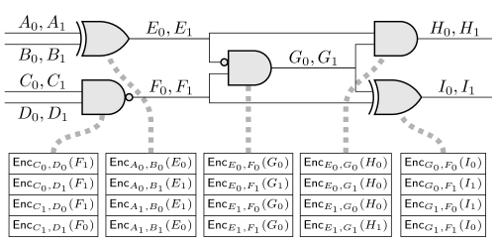
\includegraphics[width=1.0\textwidth]{Chapter2/Figs/Raster/garbledCircuit}
  \caption{Garbled Circuit example}
  \label{fig:garbledCircuit}
\end{figure}

Recent work provides optimizations to improve the computation and communication
overhead associated with encrypt/decrypt operations and ciphertext tables'
sizes. In \cite{kolesnikov2008improved30}, the authors proposed a modification
to allow XOR gates to be evaluated \textit{for free}: the labels of XOR gates
are not chosen independently but by \(\omega_{i,0} = \omega_{i,1} \xor r\), for
some random value of \(r\). Pinkas et al. \cite{pinkas2009secure38} introduced a
way to reduce the communication size of binary gates by 25\%: each gate can be
specified by three ciphertexts instead of all four. Finally,
\cite{kolesnikov2009improved29} improve some commonly used circuits such as
addition, comparision, etc., by reducing the number of non-XOR gates.

\subsection{Using GC with Homomorphic Encryption in the protocol}
\label{sec:finalcontr}
We use a standard subtractor circuit for the operation \(HD = HD' - r\): Given
a 2 n-bit bitstring, the circuit is built from 1 half-subtractor and \(n-1\)
full-subtractors as in Figure \ref{fig:substractor}, where a half-subtractor
is built from 1 XOR gate and 1 AND gate, a full-subtractor is built from 2
half-subtractors and 1 OR gate (Figure \ref{fig:fullSubstractor})

\begin{figure}[htbp!] 
  \centering    
  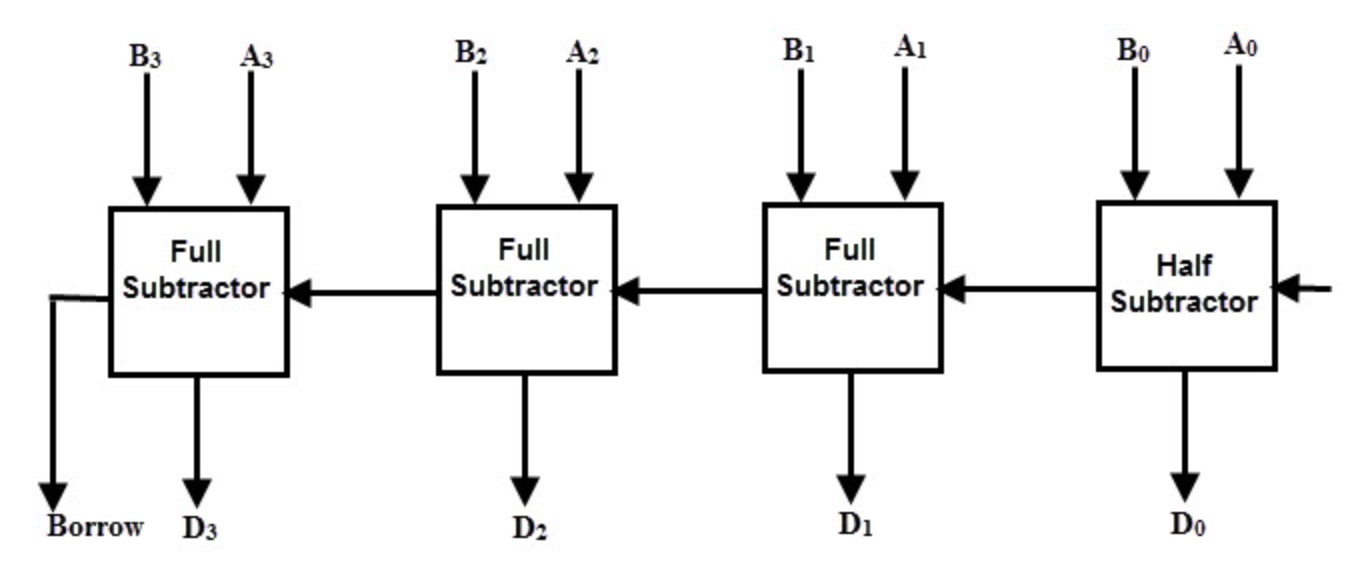
\includegraphics[width=1.0\textwidth]{Chapter7/Figs/Raster/subCircuit}
  \caption{Subtractor Circuit}
  \label{fig:substractor}
\end{figure}



\begin{figure}[htbp!] 
  \centering    
  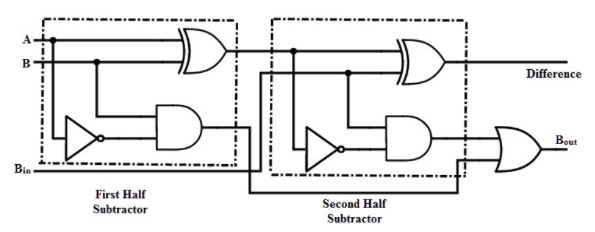
\includegraphics[width=1.0\textwidth]{Chapter7/Figs/Raster/fullSubstractor}
  \caption{Half-subtractor and Full-subtractor}
  \label{fig:fullSubstractor}
\end{figure}

In our context, let \(l\) be the bit length of the HD' and r (\(l\) is typically
10-12 bits for 1024-2048 bits biometrics data), which makes the number of
subtractor logic gates equal to \(5l\). The comparision circuit no longer needs
to output 3 results (as a standard circuits would: Either A > B, A < B or A =
B). Our aim is just to check whether \(HD' - r < \tau\), so we simply need to
have l NAND gates plus \(l-1\) XOR gates at hand for the comparison
circuit. Figure \ref{fig:comparisionCircuit1} shows an example of such a
configuration
\begin{figure}[htbp!] 
  \centering    
  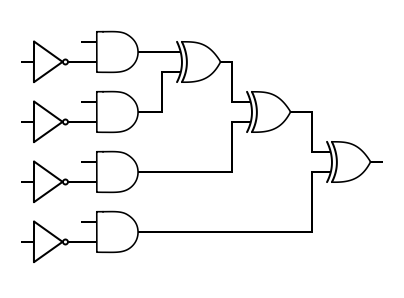
\includegraphics[scale=0.75]{Chapter7/Figs/Raster/comparisionCircuit}
  \caption{Comparator Circuit}
  \label{fig:comparisionCircuit1}
\end{figure}

\paragraph{Garbled Circuit preparation}
We denote \(GC\) to be the garbled circuit prepared by the server. The inputs to
the circuit include the server's \(GC_{r}\) and the client's \(GC_{h}\), which
are the cryptographic key \textit{labels} corresponding to the server's input
\(r\) and to the client's input \(HD'\) to the function \textit{CompareHD}. The main
function of the circuit is, first, to subtract \(HD' - r = HD\) then compare
\(HD \stackrel{?}{<} \tau\), where \(\tau\) is the constant value of the
threshold required to decide upon the authentication result, which can be built into the
circuit itself. We note that either the server or the client can play the role of
setting up the garbled circuit; in our work, we let the server take this role
(Figure \ref{fig:fourthProtocol} - Step 5, 6, 7, 8): as we have
been working on a \textit{semi-honest} server model and a \textit{malicious }
client, this will save us one proof to assess that the circuit is generated
correctly.

As pointed out previously, the server garbles the circuit \(GC\) and sends the
result to the client together with its \textit{labels} of \(r\), which are
\(K_{r_{i}}^{j}\). Next, the client uses our OT technique (discussed in the
following section) to select the correct \textit{labels} of \(HD'\): the first
part of the OT will ensure that the client will get back the encryptions
\(\enc{K_{h_{i}}^{j}}\). The second part of the OT makes sure that the protocol
is secure against \textit{malicious} clients: it needs to prove that it
decrypted and decomposed \(\enc{\mathbf{HD'}}\) correctly (Figure
\ref{fig:fourthProtocol} - Step 12,13). In other words, the client wants to
prove that the encryptions \(\enc{h_{i}}\) it sent are actually the encryptions
of the bits of \(HD'_{i}\). Recall that the server still has
\(\enc{\mathbf{HD'}}\), so the proof can be a homomorphical check of
\(\enc{\mathbf{HD'}} - \sum{2^{i}\enc{h_{i}}} = \enc{0}\). However, in order to
allow this proof to support homomorphic operations, we need to use the same
encryption scheme for the OT protocol, in other words, we need an OT protocol
based on BGV. In the next section, we discuss a this novel solution to the problem of
interfacing Garbled Circuit with Homomorphic Encryption.

We note that inside the garbled circuit, AES is normally used to encrypt the
\textit{labels}, this encryption is a part of the garbled circuit and not
related to the OT protocol we just described, and can still be used independently
to ensure the performance of circuit evaluations. Next, we discuss an approach
to design an OT protocol compatible with the BGV cryptosystem

\subsection{Oblivious Transfer}
\label{sec:obliviousTransferPre}

\textit{"You take the blue pill, the story ends. You wake up in your bed and
  believe whatever you want to believe. You take the red pill, you stay in
  wonderland, and I show you how deep the rabbit hole goes."} - Morpheus to Neo,
The Matrix.


\begin{figure}[htbp!] 
\centering    
\includegraphics[width=1.0\textwidth]{Chapter2/Figs/Raster/RedPillBluePill}
\caption[Minion]{Red Pill - Blue Pill}
\label{fig:RedPillBluePill}
\end{figure}

What if, in such situation, there were a protocol to give privacy to
\(Neo\): \(Morpheus\) should not be able to discover what option \(Neo\) has chosen. Moreover, the
protocol can also provide privacy to \(Morpheus\): \(Neo\) being thus unable to get information about the unchosen pill. In cryptography, Oblivious Transfer (OT) is a
protocol able to support such a scenario. 
In its most basic form, it is a
two-parties protocol between a \textit{Sender} and a \textit{Receiver}, denoted
by \(\begin{psmallmatrix} 2 \\ 1 \end{psmallmatrix} \)-OT. The \(Sender\) uses
two private inputs \(x_{0}, x_{1}\) and the \(Receiver\) uses one input bit
\(s\). At the completion of the protocol, the \(Receiver\) gets the bit
\(x_{s}\), without letting the \(Sender\) acquire any information about the value of
\(s\): \(\begin{psmallmatrix} 2 \\ 1 \end{psmallmatrix}
\)-OT\((x_{0},x_{1};s) = x_{s}\).

The general idea is that, when the receiver requests an item, the sender sends
all the available items to him, unaware of which one has been requested. However, the response is encrypted in such a way that the receiver
can only decrypt the one he requested. A concrete implementation example of the
\(\begin{psmallmatrix} 2 \\ 1 \end{psmallmatrix} \)-OT protocol based on
discrete log DH is illustrated in figure \ref{fig:DH21OT} (This protocol is
secure against \textit{honest but curious} attacks). The receiver picks
\(h_{0},h_{1}\) such that \(h_{0}h_{1} = h\), he cannot access both
\(\log_{g}h_{0}\) and \(\log_{g}h_{1}\). Given \(h_{0}, h_{1}\), the sender
returns ElGamal encryptions of bits \(x_{0}, x_{1}\) using \(h_{0},h_{1}\) as
public keys. The receiver then decrypts one of the encryptions to recover either
\(x_{0} \text{ or } x_{1}\)

\begin{figure}[htbp!] 
  \centering
  \procedure{DH-based Protocol}{
    \textbf{Sender} \> \> \textbf{Receiver}\\
    (x_0, x_1 \in \{0,1\}) \> \> (s \in \{0,1\})\\
    \> \> u \randomsample \mathbb{Z}n \\
    \> \> h_s \gets g^u \\
    \> \sendmessageleft*{h_0, h_1} \> h_{1 - s} \gets h/g^u \\
    u_0, u_1 \randomsample \mathbb{Z}_n \> \> \\
    (A_0, B_0) \gets (g^{u_0}, h_0^{u_0}g^{x_0}) \> \> \\
    (A_1, B_1) \gets (g^{u_1}, h_1^{u_1}g^{x_1}) \> \sendmessageright*{(A_0, B_0), (A_1, B_1)} \> x_s \gets \log_g{(B_s/A_s^u)} \\
  }
  \caption{OT protocol based on DH}
  \label{fig:DH21OT}
\end{figure}

Efficient implementations of Oblivious Transfer can be found in
\cite{naor2001efficient35}. The techniques found in \cite{ishai2003extending24}
can reduce a large number of OT protocol executions to \(\lambda\), where
\(\lambda\) is the security parameter.

\subsection{The BGV-based Oblivious Transfer protocol}
\label{sec:finalContr2}
In this thesis, we propose a new OT
technique to be used with lattice-based cryptosystems. The technique can be used
together with the garbled circuit protocol discussed earlier. The problem can be
stated as follows: Given a BGV ciphertext of a bit selection \(h_{i}\):
\(\enc{h_{i}}\), the server computes and returns a BGV encryption of the
corresponding key selected by the bit. We observe that the following homomorphic
operations will satisfy such a requirement:
\[
\enc{K_{i}^{j}} = \enc{h_{i}^{j}} \cdot \enc{K_{i}^{1}} + (1 - \enc{h_{i}^{j}}) \cdot \enc{K_{i}^{0}}
\]
where \(K_{i}^{0}, K_{i}^{1}\) are the \textit{labels} corresponding to the wire
inputs 0 or 1. The function includes one level of homomorphic multiplication, two
additions and one multiplication with a constant. This approach is simple enough
and it is secure against a \textit{malicious client} model in our context because
the client needs to prove that he actually encrypted \(\enc{h_{i}}\)
correctly already. Other applications of this OT should take into account that a
malicious client can encrypt \(\enc{h_{i}}\) incorrectly to obtain information about
\(K_{i}^{0}\) and/or \(K_{i}^{1}\).

The other issue that we have to be careful about is \textit{Circuit Privacy}:
for a multi-factor attacker able to access the secret key but not the
biometric template, it is possible to obtain information about the randomness of the
operation. The randomness of the above operation is of the form
\(K_{i}^{0} + (K_{i}^{1} - K_{i}^{0})r_{0}\), which is correlated to both
keys. Again, we can mask the randomness of this leakage similarly to what we did
in the second variant of the protocol. By a similar analysis, we can still show
that computing the HD cannot be achieved with a significant level of probability (the privacy
security requirement related to what the client sees is indistinguishable
from the probability he has to compute the HD, which is not much more than random
guessing).

% \begin{figure}[h!]
%   \centering
%   \begin{equation*}
%     \begin{array}{c c c}
%       \text{\textbf{Sender}} & & \text{\textbf{Receiver}} \\
%       \\
%       (x_{0}, x_{1} \in \{0,1\}) & & (s \in \{0,1\}) \\
%                              & & u \randomsample \mathbb{Z}_{n}\\
%                              & & h_{s} \gets g^{u}\\
%                              & & h_{1-s} \gets h/g^{u}\\
%                              & \xleftarrow{h_{0}, h_{1}} & \\
%       u_{0}, u_{1} \randomsample \mathbb{Z}_{n} & & \\
%       (A_{0}, B_{0}) \gets (g^{u_{0}}, h_{0}^{u_{0}}g^{x_{0}}) & & \\
%       (A_{1}, B_{1}) \gets (g^{u_{1}}, h_{1}^{u_{1}}g^{x_{1}}) & & \\
%                              & \xrightarrow{(A_{0}, B_{0}),(A_{1}, B_{1})} & \\
%       & & x_{s} \gets \log_{g}(B_{s}/A_{s}^{u})
%     \end{array}
%   \end{equation*}
%   \caption{OT protocol based on DH}
%   \label{fig:DH21OT}
% \end{figure}



\section{The details}
\label{sec:4thProcDetails}

\subsection{The protocol description}
\label{sec:4thprocSteps}
With a notation similar to the one used for previous protocols, we describe the last variant of the authentication system as follows (Figure \ref{fig:fourthProtocol})
\begin{enumerate}
\item In the enrollment stage, the client $\user$ extracts his template $\enc{\mathbf{T}}$ and sends it to the server $\server$
\item In the authentication stage, $\user$ extracts his query template $\enc{\mathbf{Q}}$ and sends it to the server
\item $\user$ uses a Schnorr-based ZKP (Section \ref{sec:zkpschnorr}) to prove that the noise associated with $\enc{\mathbf{Q}}$ is small
\item $\user$ uses the Challenge-Response technique (Section \ref{sec:challengeResponse}) to prove that $\enc{\mathbf{Q}}$ is encrypting a binary message
\item If the proofs pass, $\server$ starts preparing the garbled circuit $GC$, it first samples $r \randomsample \mathbb{Z}_{t}$ and decomposes it into a binary representation, assuming that $r$ is $k$ bits long.
\item $\server$ establishes $k$ pair of keys $(K_{r_{i}}^{0}, K_{r_{i}}^{1})$ for the inputs of $GC_{r}$
\item $\server$ establishes $k$ pair of keys $(K_{h_{i}}^{0}, K_{h_{i}}^{1})$ for the inputs of $GC_{h}$
\item $\server$ establishes the pair of keys for authentication result outputs $(K_{out}^{0}, K_{out}^{1})$
\item $\server$ encrypts the $k$ keys of $GC_{h}$ to obtain $\enc{K_{h_{i}}^{0}}, \enc{K_{h_{i}}^{1}}$
\item $\server$ computes $\enc{HD} \gets HDBGV(\enc{\mathbf{T}}, \enc{\mathbf{Q}})$
\item $\server$ masks the Hamming Distance $\enc{\mathbf{HD'}} = \enc{\mathbf{HD + r}}$ and sends the result together with the garbled circuit $GC$ and the keys $K_{r_{i}}^{j}$ to $\user$, where $j$ associates the key of $GC_{r}$ corresponding to the $r$ chosen by $\server$.
\item $\user$ decrypts $\enc{\mathbf{HD}'}$
\item $\user$ decomposes the plaintext $HD'$ into its binary representation $HD' = \sum_{0}^{k-1}2^{i}h_{i}$
\item $\user$ re-encrypts the bits of the decomposition
\item $\user$ uses the ciphertext $\enc{h_{i}}$ in the Oblivious Transfer Protocol (Section \ref{sec:obliviousTransferPre}) to retrieve the ciphertexts $\enc{K_{h_{i}}^{j}}$
\item $\user$ decrypts the result to obtain another set of keys for the garbled circuit
\item $\user$ evaluates the circuit with the keys $(K_{h_{i}}^{j}, K_{r_{i}}^{j})$ and sends the result to the server
\item $\server$ compares this outcome with the output keys prepared in step 8 and outputs the final authentication result.
\end{enumerate}

\begin{figure}[htbp!] 
  \centering \procedure{The Fourth Protocol}{
    \textbf{Client} \> \> \textbf{Server}\\
    \text{1. Registered template \textbf{T}} \> \sendmessageright*{\enc{\mathbf{T}}} \> \text{Store } \enc{\mathbf{T}}\\
    \text{2. Query template \textbf{Q}} \> \sendmessageright*{\enc{\mathbf{Q}}} \> \text{Initiate Query Proof}\\
    \> \sendmessageleft*{\text{3. Prove small noise in \textbf{Q}}} \> \\
    \> \sendmessageleft*{\text{4. Prove \textbf{Q} is binary}} \> \\
    \> \> \text{Sample \(r \randomsample \mathbb{Z}_{t}\)}\\
    \> \> \text{5. Setup garbled circuit GC, for } i = 1,\dots,k \\
    \> \> \text{6. Setup } (K^{0}_{r_{i}}, K^{1}_{r_{i}}) \text{ for } GC_r \\
    \> \> \text{7. Setup } (K^{0}_{h_{i}}, K^{1}_{h_{i}}) \text{ for } GC_{h}\\
    \> \> \text{8. Setup } (K^{0}_{out}, K^{1}_{out}) \\
    \> \> \text{9. Compute } \enc{K^0_{h_i}},\enc{K^1_{h_i}}\\
    \> \> \text{10. } \enc{\mathbf{HD}} = HDBGV(\enc{\mathbf{T}},\enc{\mathbf{Q}}) \\
    \> \> \text{Compute } \enc{\mathbf{HD'}} = \enc{\mathbf{HD + r}}\\
    \> \sendmessageleft*{\enc{\mathbf{HD'}}} \> \\
    \> \sendmessageleft*{GC} \> \\
    \> \sendmessageleft*{K_{r_i}^j \text{of } GC_r} \> \\
    \text{12. Decrypt } \mathbf{HD'} = dec(\enc{\mathbf{HD}}) \> \> \\
    \text{13. Decompose } \mathbf{HD'} = \sum_{i=0}^k{2^ih_i} \> \> \\
    \text{14. Encrypt } \enc{h_i} \> \> \\
    \text{15. Initiate OT protocol} \> \> \\
    \> \sendmessageright*{16. \enc{h_i}} \> \\
    \> \sendmessageright*{\text{17. Prove correct decryption}} \> \\
    \> \sendmessageleft*{\text{18. Retrieve } \enc{K_{h_i}^j}} \> \\
    \text{19. Decrypt } K_{h_i}^j \> \> \\
    20. K_{out} = GC( K_{h_i}^j , K_{r_i}^j) \> \> \\
    \> \sendmessageright*{K_{out}} \> \text{21. Compare } K_{out} \text{ with } K_{out}^0, K_{out}^1 \\
    \> \> \text{ Output res = \textbf{Accept|Reject}}
  }
  \caption{The fourth Protocol}
  \label{fig:fourthProtocol}
\end{figure}

\subsection{Implementation Result}
\label{sec:7result}
We observe significant improvements in communication size thanks to the
Challenge-Response technique (only 2 messages required). The Schnorr-based ZKP
also contributes to this factor by reducing the number of rounds in proofs to 1,
instead of 17 for similar settings
$(n = 2048, t = 2048, \alpha q = 8, q \approx 2^{72}, FAR \approx
10^{-3})$. The total number of gates used in the garbled circuit for $n=2048$ equals 25, which only cost $\approx 3.2$ KB for the HD comparison purpose. All of
these improvements come with a one time setup cost for preparing the switch keys
for the HD computation operation: we need to rotate 10 times and swap 1 time to
compute $HD$, each operation needs 1 key switch to transform the result back to
the original ciphertext format (2 ring elements) before the next homomorphic
operation. The total key switch size needed is $2*n*\log q*11$, which is
approximately 389 MB in our setting. Considering the privacy features provided,
we believe such one time set up cost is acceptable. We conclude the chapter with
the comparison of the 4 protocols described in the thesis

\begin{table}[h!]
\centering
\caption{Protocols' features comparison}
\label{my-label}
\begin{tabular}{lllll}
\hline
                                          & \textbf{Multi-factor}    & \textbf{HD Non-exposure} & \textbf{Low Init cost} & \textbf{Low Communication} \\ \hline
\multicolumn{1}{|l|}{\textbf{Protocol 1}} & \multicolumn{1}{l|}{No}  & \multicolumn{1}{l|}{No}        & \multicolumn{1}{l|}{Yes}   & \multicolumn{1}{l|}{Yes}   \\ \hline
\multicolumn{1}{|l|}{\textbf{Protocol 2}} & \multicolumn{1}{l|}{Yes} & \multicolumn{1}{l|}{No}        & \multicolumn{1}{l|}{Yes}   & \multicolumn{1}{l|}{Yes}   \\ \hline
\multicolumn{1}{|l|}{\textbf{Protocol 3}} & \multicolumn{1}{l|}{Yes} & \multicolumn{1}{l|}{Yes}       & \multicolumn{1}{l|}{Yes}   & \multicolumn{1}{l|}{No}    \\ \hline
\multicolumn{1}{|l|}{\textbf{Protocol 4}} & \multicolumn{1}{l|}{Yes} & \multicolumn{1}{l|}{Yes}       & \multicolumn{1}{l|}{No}    & \multicolumn{1}{l|}{Yes}   \\ \hline
\end{tabular}
\end{table}
    
% \begin{figure}[h!]
%   \centering
%     \begin{equation*}
%         \begin{array}{c c c}
%         \text{\textbf{Client}} & & \text{\textbf{Server}} \\
%           \\
%           \text{1. Registered template \textbf{T}} & \xrightarrow{\enc{\mathbf{T}}} & \text{Store } \enc{\mathbf{T}}\\
          
%           \text{2. Query template \textbf{Q}} & \xrightarrow{\enc{\mathbf{Q}}} & \text{Initiate Query Proof}\\

%                                & \xleftrightarrow{\text{3. Prove small noise in \textbf{Q}}} & \\

%                                & \xleftrightarrow{\text{4. Prove \textbf{Q} is binary}} & \\

%                                & & \text{Sample \(r \randomsample \mathbb{Z}_{t}\)}\\
%                                & & \text{5. Setup garbled circuit GC, for } i = 1,\dots,k \\

%                                & & \text{6. Setup } (K^{0}_{r_{i}}, K^{1}_{r_{i}}) \text{ for } GC_r \\
          
%                                & & \text{7. Setup } (K^{0}_{h_{i}}, K^{1}_{h_{i}}) \text{ for } GC_{h}\\
          
%                                & & \text{8. Setup } (K^{0}_{out}, K^{1}_{out}) \\

%                                & & \text{9. Compute } \enc{K^0_{h_i}},\enc{K^1_{h_i}}\\
%           \\

%                                & & \text{10. } \enc{\mathbf{HD}} = HDBGV(\enc{\mathbf{T}},\enc{\mathbf{Q}}) \\
          
%                                    & & \text{Compute } \enc{\mathbf{HD'}} = \enc{\mathbf{HD + r}}\\

%                                & \xleftarrow{\enc{\mathbf{HD'}}} & \\

%                                & \xleftarrow{GC} & \\

%                                & \xleftarrow{K_{r_i}^j \text{of } GC_r} & \\

%           \text{12. Decrypt } \mathbf{HD'} = dec(\enc{\mathbf{HD}}) & & \\

%           \text{13. Decompose } \mathbf{HD'} = \sum_{i=0}^k{2^ih_i} & & \\

%           \text{14. Encrypt } \enc{h_i} & & \\
          
%           \text{15. Initiate OT protocol} & & \\

%                                & \xrightarrow{16. \enc{h_i}} & \\
          
%                                & \xrightarrow{\text{17. Prove correct decryption}} & \\

%                                & \xleftarrow{\text{18. Retrieve } \enc{K_{h_i}^j}} & \\

%           \text{19. Decrypt } K_{h_i}^j & & \\
%           20. K_{out} = GC( K_{h_i}^j , K_{r_i}^j) & & \\

%                                & \xrightarrow{K_{out}} & \text{21. Compare } K_{out} \text{ with } K_{out}^0, K_{out}^1 \\
%           & & \text{ Output res = \textbf{Accept|Reject}}
%         \end{array}
%     \end{equation*}

%   \caption{The fourth protocol}
%   \label{fig:fourthProtocol}
% \end{figure}


% \section{Related Work}
% \label{sec:chap7RelatedWorks}



% Consider the following situation:  How can he achieve that?
% Suppose that the plaintext \(P\) is encoded as coefficients of a polynomial, or
% specifically, \(P\) can be an element of the ring \(R_{2}\), where
% \(R_{2} = \frac{\mathbb{Z}_{2}[x]}{x^{n} + 1}\), this ring has been used by many
% RLWE based cryptosystems lately. One solution can be to apply the Zero Knowlege
% Proof technique. This is however a costly choice. There are mainly two
% approaches for ZKP, the Schnorr's based protocol,
% e.g. \cite{benhamouda2014better} or a Stern's based protocol such as
% \cite{stern1993new} or \cite{ling2013improved}. The first approach has
% limitations on the norm of the secret it can prove and cannot be used to prove
% the knowledge of binary messages with norm 2. The second approach can prove
% binary messages but it has a very high communication cost due to a roundness
% error equaling \(2/3\).
% \subsection{ZKP and $\sum$-Protocol}
% \label{sub:zkp_and_sum_protocol}
% A Zero-Knowledge Proof of Knowledge (ZKPoK) is a two party protocol between a
% Prover $P$ and a Verifier $V$. The protocol allows $P$ to convince $V$ that it
% knows some secret without revealing anything about the secret. We refer readers
% to \cite{bellare1992defining} for formal definition of the original ZKPoK. 

% Notation: 




% \subsection{Schnorr-based ZKP technique}
% \label{sec:zero-knowledge-proof}


% \begin{figure}[htbp!] 
%   \centering \procedure{AND-Composition of Benhamouda ZKP}{
%     \textbf{Prover} \> \> \textbf{Verifier}\\
%     \mathbf{r_s,r_{e_0},r'_{s},r'_{e_{0}}} \randomsample D_{\beta_0} \> \> \\
%     \mathbf{r_e,r'_{e}} \randomsample D_{\beta} \> \> \\
%     \mathbf{r_m,r'_{m}} \randomsample D_{t} \> \> \\
%     \mathbf{t_c} = \mathbf{-c_1r_s} + t\mathbf{r_e + r_m} \> \> \\
%     \mathbf{t_k} = \mathbf{-p_1r_s} - t\mathbf{r_{e_0}} \> \> \\
%     \mathbf{t'_c} = \mathbf{-c_1r'_s} + t\mathbf{r'_e + r'_m} \> \> \\
%     \mathbf{t'_k} = \mathbf{-p_1r'_s} - t\mathbf{r'_{e_0}} \> \> \\
%     (c_{aux}, d_{aux}) = aCommit(\mathbf{t_c,t_k}) \> \> \\
%     (c'_{aux}, d'_{aux}) = aCommit(\mathbf{t'_c,t'_k}) \>
%     \sendmessageright*{c_{aux},c'_{aux}} \> \\
%     \> \> c \randomsample \mathcal{C} = \left\{ 0,\dots, 2n -1  \right\}\\
%     \>  \sendmessageleft*{c} \> \\
%     \mathbf{s_s = r_s + x^cs},\mathbf{s'_s = r'_s + x^cs} \> \> \\
%     \mathbf{s_e = r_e + x^ce},\mathbf{s'_e = r'_e + x^ce} \> \> \\
%     \mathbf{s_m = r_m + x^cm},\mathbf{s'_m = r'_m + x^cm} \> \> \\
%     \mathbf{s_{e_0} = r_{e_0} + x^ce_0},\mathbf{s'_{e_0} = r'_{e_0} + x^ce_0} \> \> \\
%     \> \sendmessageright{top=$d_{aux}$, bottom=$d'_{aux}$} \> \\
%     \> \> \mathbf{x^cc_0} + \mathbf{t_c} \stackrel{?}{=} -\mathbf{c_1s_s} + t\mathbf{s_e} + \mathbf{s_m}\\
%     \> \> \mathbf{x^cc_0} + \mathbf{t'_c} \stackrel{?}{=} -\mathbf{c_1s'_s} + t\mathbf{s'_e} + \mathbf{s'_m}\\
%     \> \> \mathbf{x^cp_0} + \mathbf{t_k} \stackrel{?}{=} -\mathbf{p_1s_s} - t\mathbf{s_{e_0}}\\
%     \> \> \mathbf{x^cp_0} + \mathbf{t'_k} \stackrel{?}{=} -\mathbf{p_1s'_s} - t\mathbf{s'_{e_0}}\\
%     \> \> aCOpen(\mathbf{t_c, t_k}, c_{aux}, d_{aux}) \stackrel{?}{=} accept \\
%     \> \> aCOpen(\mathbf{t'_c, t'_k}, c'_{aux}, d'_{aux}) \stackrel{?}{=} accept \\
%     \> \> \norm{s_s}, \norm{s_{e_0}},\norm{s'_s}, \norm{s'_{e_0}} \leq 2\beta_0 \\
%     \> \> \norm{s_e},\norm{s'_e}  \leq 2\beta \\
%     \> \> \norm{s_m},\norm{s'_m} \leq 2t
%   }
%   \caption{AND-Composition for ZKP-BV}
%   \label{fig:belhamoudaProtocolAND}
% \end{figure}

  % \begin{figure}[h!]
  %   \centering
  %   \begin{equation*}
  %     \begin{array}{c c c}
  %       \text{\textbf{Prover}} & & \text{\textbf{Verifier}} \\
  %       \\
  %       \mathbf{r_s,r_{e_0},r'_{s},r'_{e_{0}}} \randomsample D_{\beta_0} & & \\
  %       \mathbf{r_e,r'_{e}} \randomsample D_{\beta} & & \\
  %       \mathbf{r_m,r'_{m}} \randomsample D_{t} & & \\
  %       \mathbf{t_c} = \mathbf{-c_1r_s} + t\mathbf{r_e + r_m} & & \\
  %       \mathbf{t_k} = \mathbf{-p_1r_s} - t\mathbf{r_{e_0}} & & \\
  %       \mathbf{t'_c} = \mathbf{-c_1r'_s} + t\mathbf{r'_e + r'_m} & & \\
  %       \mathbf{t'_k} = \mathbf{-p_1r'_s} - t\mathbf{r'_{e_0}} & & \\
  %       (c_{aux}, d_{aux}) = aCommit(\mathbf{t_c,t_k}) & & \\
  %       (c'_{aux}, d'_{aux}) = aCommit(\mathbf{t'_c,t'_k}) &
  %                                                        \xrightarrow{\hspace{1em}c_{aux},c'_{aux}\hspace{1em}} & \\
  %                              & & c \randomsample \mathcal{C} = \left\{ 0,\dots, 2n -1  \right\}\\
  %                              &  \xleftarrow{\hspace{1em}c\hspace{1em}} & \\
  %       \mathbf{s_s = r_s + x^cs},\mathbf{s'_s = r'_s + x^cs} & & \\
  %       \mathbf{s_e = r_e + x^ce},\mathbf{s'_e = r'_e + x^ce} & & \\
  %       \mathbf{s_m = r_m + x^cm},\mathbf{s'_m = r'_m + x^cm} & & \\
  %       \mathbf{s_{e_0} = r_{e_0} + x^ce_0},\mathbf{s'_{e_0} = r'_{e_0} + x^ce_0} & & \\
  %                              & \xrightarrow[\hspace{1em}d'_{aux}, \mathbf{t'_c, t'_k, s'_s, s'_e, s'_m,
  %                                s'_{e_0}}\hspace{1em}]{\hspace{1em}d_{aux}, \mathbf{t_c, t_k, s_s, s_e, s_m,
  %                                s_{e_0}}\hspace{1em}} & \\
  %                              & & \mathbf{x^cc_0} + \mathbf{t_c} \stackrel{?}{=} -\mathbf{c_1s_s} + t\mathbf{s_e} + \mathbf{s_m}\\
  %                              & & \mathbf{x^cc_0} + \mathbf{t'_c} \stackrel{?}{=} -\mathbf{c_1s'_s} + t\mathbf{s'_e} + \mathbf{s'_m}\\
  %                              & & \mathbf{x^cp_0} + \mathbf{t_k} \stackrel{?}{=} -\mathbf{p_1s_s} - t\mathbf{s_{e_0}}\\
  %                              & & \mathbf{x^cp_0} + \mathbf{t'_k} \stackrel{?}{=} -\mathbf{p_1s'_s} - t\mathbf{s'_{e_0}}\\
  %                              & & aCOpen(\mathbf{t_c, t_k}, c_{aux}, d_{aux}) \stackrel{?}{=} accept \\
  %                              & & aCOpen(\mathbf{t'_c, t'_k}, c'_{aux}, d'_{aux}) \stackrel{?}{=} accept \\
  %                              & & \norm{s_s}, \norm{s_{e_0}},\norm{s'_s}, \norm{s'_{e_0}} \leq 2\beta_0 \\
  %                              & & \norm{s_e},\norm{s'_e}  \leq 2\beta \\
  %                              & & \norm{s_m},\norm{s'_m} \leq 2t
  %     \end{array}
  %   \end{equation*}
  %   \caption{AND-Composition for ZKP-BV }
  %   \label{fig:belhamoudaProtocolAND}
  % \end{figure}


% \subsection{Combination of ZKP}
% \label{sec:combination-zkp}
% A $\sum-$protocol can be composed together to construct more complex relations.
% There are several forms of decomposition such as AND, OR, NEQ, etc.  We describe
% some forms of composition of the \(\sum-protocol\) that are used in our own protocol:
% AND-composition, OR-composition. We first describe the generic \(\sum-\)protocol
% and its combinations. The BV-ZKP (Figure \ref{fig:belhamoudaProtocol}) protocol
% is an instance of such a protocol and the technique can be applied inherently.
% \begin{description}
% \item[$\sum-$protocol] The protocol is a generic 3-moves transaction between 2 parties
%   \(Prover\) and \(Verifier\), it is used to prove (supporting zero-knowledge) a
%   relation \(R(x,w)\), where \(x\) is the public parameter known by both
%   parties and \(w\) is a witness known by the \(Prover\) only. The protocol's
%   view is a set of 3 messages (Figure \ref{fig:sigmaProtocol}): the commitment
%   \(c\) is a function of a random factor \(\rho\), the challenge \(ch\) is
%   normally random, and the response \(r\) is a function computed from
%   \(x, w, \rho, ch\). There are 2 extra algorithms for the \(\sum-\)protocol: a
%   \(verify(r,ch,c)\) algorithm used by the \(Verifier\) in the last step to
%   check the correctness of the proof result, and a simulator \(sim\), taking
%   \(x\) and a random parameter \(\rho'\) as inputs, and and outputting a view
%   \(\bar{c},\bar{ch},\bar{r}\) that is indistinguishable from the genuine view
%   of the protocol.

%   \begin{figure}[htbp!] 
%     \centering \procedure{Sigma Protocol}{
%       \textbf{Prover} \> \> \textbf{Verifier}\\
%       \rho \randomsample random \> \> \\
%       c \gets comm(\rho) \> \> \\
%       \> \sendmessageright*{c} \> \\
%       \> \> ch \randomsample random \\
%       \> \sendmessageleft*{ch} \> \\
%       r \gets resp(\rho,w,x,ch) \> \> \\
%       \> \sendmessageright*{r} \> \\
%       \> \> verify(r, ch, c)\\
%     }
%     \caption{Sigma Protocol}
%     \label{fig:sigmaProtocol}
%   \end{figure}
%   % \begin{figure}[h!]
%   %   \centering
%   %   \begin{equation*}
%   %     \begin{array}{c c c}
%   %       \text{\textbf{Prover}} & & \text{\textbf{Verifier}} \\
%   %       \\
%   %       \rho \randomsample random & & \\
%   %       c = comm(\rho) & & \\
%   %                              & \xrightarrow{c} & \\
%   %                              & & ch \randomsample random \\
%   %                              & \xleftarrow{ch} & \\
%   %       r = resp(\rho,w,x,ch) & & \\
%   %                              & \xrightarrow{r} & \\
%   %                              & & verify(r, ch, c)\\
%   %     \end{array}
%   %   \end{equation*}
%   %   \caption{Sigma Protocol}
%   %   \label{fig:sigmaProtocol}
%   % \end{figure}
% \end{description}


% \begin{description}
% \item[AND-COMPOSITION] Given two relations $R_1 = \left\{ (v_1,w_1) \right\}$
%   and $R_2 = \left\{ (v_2, w_2) \right\}$ with the same challenge space, a
%   $\sum$-Protocol of
%   $R_1 \wedge R_2 = \left\{ (v_1, v_2, w_1, w_2): (v_1;w_1) \in R_1, (v_2,w_2)
%     \in R_2\right\}$ can be obtained by running a $\sum$-Protocol for $R_1$ and
%   a $\sum$-Protocol for $R_2$ in parallel, using a \emph{common} challenge.
%   Figure \ref{fig:belhamoudaProtocolAND} is a concrete example combining 2 ZKP for BV.
  

% \item[OR-Compostion] In this composition, given the $\sum-protocol$ for many  
%   relations $R_{1}$,$R_{2}$,\dots,\(R_{n}\) the goal is to construct a protocol for the
%   relation
%   $R_{OR}(\vec{x}, w_{i}) $, where \(\exists i \leq n: R(x_{i},w_{i}) = 1\). The main reason behind this composition is that the verifier
%   can let the prover use the simulator of the \(\sum-protocol\) for the
%   relations \(R_{j}\), for which the prover does not know the witness.
%   The verifier provides a single challenge \(c\)
%   such that the prover can split that into challenges \(c_{1}, c_{2}, \dots, c_{n}\)
%   provided that \(c_{i}\) satisfies a linear constraint in terms of \(c\),
%   for example \(c = c_{1} \xor c_{2} \xor \dots \xor c_{n}\). The final OR-combination proof is
%   obtained by composing one run of the \(\sum-protocol\) with other runs of the
%   simulators for the \(\sum-protocol\). (Figure \ref{fig:OR-Combination})

%   \begin{figure}[htbp!] 
%     \centering \procedure{OR Composition of ZKP}{
%       \textbf{Prover} \> \> \textbf{Verifier}\\
%       \rho_{i} \randomsample random \> \> \\
%       c_{i} = comm(\rho_{i}) \> \> \\
%       \text{For } j = 1,\dots,n \wedge j \neq i: \> \> \\
%       \text{    } \rho_{j} \randomsample random; \> \> \\
%       \text{    } (c_{j}, ch_{j}, r_{j}) \gets ZKPSim(\rho_{j}, x_{j}) \> \> \\
%       \> \sendmessageright*{ch_j,c_{1}, c_{2}, \dots, c_{n}} \> \\
%       \> \> ch \randomsample \mathbb{Z}_{n} \\
%       \> \sendmessageleft*{ch} \> \\
%       ch_{i} = ch - \sum_{j \neq i}{ch_{j}} \> \> \\
%       r_{i} = resp(\rho_{i}, w_{i}, x_{i}, ch_{i}) \> \> \\
%       \> \sendmessageright*{r_{1}, r_{2}, \dots, r_{n}} \> \\
%       \> \> \forall i \in [n], ver(r_{i}, ch_{i}, c_{i}) = 1 \\
%       \> \> ch = \sum_{i \in [n]}ch_{i}\\
%     }
%     \caption{OR Composition of ZKP}
%     \label{fig:OR-Composition}
%   \end{figure}
  % \begin{figure}[h!]
  %   \centering
  %   \begin{equation*}
  %     \begin{array}{c c c}
  %       \text{\textbf{Prover}} & & \text{\textbf{Verifier}} \\
  %       \\
  %       \rho_{i} \randomsample random & & \\
  %       c_{i} = comm(\rho_{i}) & & \\
  %       \text{For } j = 1,\dots,n \wedge j \neq i: & & \\
  %       \text{    } \rho_{j} \randomsample random; & & \\
  %       \text{    } (c_{j}, ch_{j}, r_{j}) \gets ZKPSim(\rho_{j}, x_{j}) & & \\
  %                              & \xrightarrow[ch_{j}]{c_{1}, c_{2}, \dots, c_{n}} & \\
  %                              & & ch \randomsample \mathbb{Z}_{n} \\
  %                              & \xleftarrow{ch} & \\
  %       ch_{i} = ch - \sum_{j \neq i}{ch_{j}} & & \\
  %       r_{i} = resp(\rho_{i}, w_{i}, x_{i}, ch_{i}) & & \\
  %                              & \xrightarrow{r_{1}, r_{2}, \dots, r_{n}} & \\
  %                              & & \forall i \in [n], ver(r_{i}, ch_{i}, c_{i}) = 1 \\
  %                              & & ch = \sum_{i \in [n]}ch_{i}\\
  %     \end{array}
  %   \end{equation*}
  %   \caption{}
  %   \label{fig:OR-Combination}
  % \end{figure}
% \end{description}





%%% Local Variables:
%%% mode: latex
%%% TeX-master: "../thesis"
%%% End:

% \subsection*{Summary of previous work}
% \begin{description}
% \item Lyubashevsky's proof systems (\cite{lyubashevsky2008lattice},
%   \cite{lyubashevsky2009fiat}): This system is similar to the classical Schnorr's
%   ZKP system, the main advantage is its communication size efficiency. However,
%   this approach is not zero-knowledge (it is only proved to be witness
%  -indistinguishable). Moreover, there is a completeness error in each round, and
%   lastly, the extraction gap is $O(\sqrt{n})$.

%   A quick discussion on extraction gaps: we refer to an extraction gap as a security
%   parameter of ZKP systems for ISIS problem. Generally, we say that a proof accepts
%   an extraction gap $\gamma$ ($\gamma > 1$) if the knowledge extractor of the
%   protocol can extract a vector $\vec{v}$ such that
%   $\norminf{v} = \gamma \norminf{w}$, where $\norminf{w}$ is a valid witness
%   from the \emph{Prover}. Ideally, when $\gamma = 1$, one can use the extractor
%   to solve the underlying ISIS instance. In other words, ZKP with $\gamma = 1$
%   is strongly secure, as breaking it is at least as hard as solving the
%   underlying problem. When $\gamma > 1$, the soundness of the proof has to rely
%   on a stronger hardness assumption of certain potentially easier problems is hard
%   to solve.
% \item Micciancio-Vadhan proof system \cite{micciancio2003statistical}: This
%   protocol provides ZKP for the GapCVP problem, but it can be adapted to prove the ISIS
%   relation: Let $\mathbf{B}$ be a basis of the perp lattice
%   $\Lambda_q^\bot(\mathbf{A}) = \{\mathbf{x} \in \mathbb{Z}^m: \mathbf{A.x = 0}\
%   \mod \ q\}$.  and $\mathbf{t} \in \mathbb{Z}^m: \mathbf{A.t = y}\ \mod \ q$
%   ($\mathbf{B}$ and $\mathbf{t}$ can be computed efficiently), then run the ZKP
%   protocol for $GapCVP_\gamma^\infty$ with public parameters
%   $(\mathbf{B,t},\beta$). The $Prover$'s witness is $\mathbf{e = t - x}$. Recall
%   that The knowledge extractor of the protocol can output a vector
%   $\mathbf{e'} \in \Lambda_q^\bot( \mathbf{A}$ such that
%   $\norminf{\mathbf{ t - e'}} \leq g.\beta$ for some $g \geq O(\sqrt[]
%   {m}$). This implies a perfect ZKPoPK with extraction gap $O(\sqrt[]{m})$.
% \item Stern's protocol [\todo{citeStern}] and extension: The original Stern's
%   proof worked on the SD relation \todo{SD relation}. This ZKP does not have any
%   completeness error and there is no extraction gap, i.e., $\gamma =
%   1$. Extensions of this work include KTX [137,85], associated with the
%   following relation \todo{ktxRelation}.

%   The work of \cite{ling2013improved} provides a proof for the ISIS relation
%   \todo{ISIS relation}.  Stern's based techniques inherently do not have
%   extraction gaps nor completeness errors, their communication efficiency is:
%   \todo{missing figure}. Our protocol will also be based on this technique, the
%   enhancement being that it can prove different bounds of different elements in the
%   $Prover$'s witness vector. Such improvement is important in ZKPoPK for
%   lattice-based cryptosystems, especially in contexts where public key settings
%   and homomorphic operations are used. The bounds of messages and errors can be
%   largely different: for example, the original message can be binary while the
%   noises' bounds increase according to the ladder of homomorphic operations.

% \end{description}






%%% Local Variables:
%%% mode: latex
%%% TeX-master: "../thesis"
%%% End:
